\chapter{深度学习}\label{chapter:7}
现在让我们开始学习深度学习。在本部分中,将概述神经网络,讨论向量化,并讨论使用反向传播训练神经网络。

\section{使用非线性模型的监督学习}\label{sec:7.1}

在监督学习设置中(从输入 $x$ 预测 $y$),假设我们的模型/假设是 $h_\theta(x)$。过去的章节里考虑了 $h_\theta(x) = \theta^T x$(线性回归)或 $h_\theta(x) = \theta^T \phi(x)$(其中 $\phi(x)$ 是特征映射)的情况。这两个模型的共同点是它们在参数 $\theta$ 中是线性的。接下来,我们将考虑学习在参数 $\theta$ 和输入 $x$ 中都\textbf{非线性 (non-linear)}的一般模型族。最常见的非线性模型是神经网络,我们将在下一节开始定义。对于本节,将 $h_\theta(x)$ 视为抽象的非线性模型即可。\footnote{如果需要一个具体的例子,可以考虑模型 $h_\theta(x) = \theta_1^2 x_1^2 + \theta_2^2 x_2^2 + \dots + \theta_d^2 x_d^2$,尽管它不是神经网络。}

假设 $\{(x^{(i)}, y^{(i)})\}_{i=1}^n$ 是训练样本。我们将定义非线性模型及其学习的损失/成本函数。

\subsection*{回归问题}

为简单起见,我们从输出是实数的情况开始,即 $y^{(i)} \in \mathbb{R}$,因此模型 $h_\theta(x)$ 也输出实数 $h_\theta(x) \in \mathbb{R}$。将学习第 $i$ 个样本 $(x^{(i)}, y^{(i)})$ 的最小二乘成本函数定义为
\begin{equation} \label{eq:7.1}
    J^{(i)}(\theta) = \frac{1}{2} (h_\theta(x^{(i)}) - y^{(i)})^2,
\end{equation}
数据集的均方成本函数定义为
\begin{equation} \label{eq:7.2}
    J(\theta) = \frac{1}{n} \sum_{i=1}^n J^{(i)}(\theta),
\end{equation}
这与线性回归中的定义相同,只是为了与约定一致,我们在成本函数前引入了常数 $1/n$。注意,将成本函数乘以一个标量不会改变成本函数的局部最小点或全局最小点。另请注意,尽管成本函数的形式也是均方损失,但 $h_\theta(x)$ 的参数化与线性回归的情况不同。在后文中,“损失”和“成本”这两个词会互换使用。

\subsection*{二元分类}
接下来定义二元分类的模型和损失函数。假设输入 $x \in \mathbb{R}^d$。令 $\bar{h}_\theta: \mathbb{R}^d \to \mathbb{R}$ 是一个参数化模型(逻辑线性回归中 $\theta^T x$ 的类比)。将输出 $\bar{h}_\theta(x) \in \mathbb{R}$ 称为 logit。类似于第 \ref{sec:2.1} 节,使用 logistic 函数 $g(\cdot)$ 将 logit $\bar{h}_\theta(x)$ 转换为概率 $h_\theta(x) \in [0, 1]$:
\begin{equation} \label{eq:7.3}
    h_\theta(x) = g(\bar{h}_\theta(x)) = 1 / (1 + \exp(-\bar{h}_\theta(x))).
\end{equation}
使用以下方式建模给定 $x$ 和 $\theta$ 的 $y$ 的条件分布:
\[
\begin{aligned}
    P(y = 1 \mid x; \theta) &= h_\theta(x) \\
    P(y = 0 \mid x; \theta) &= 1 - h_\theta(x)
\end{aligned}
\]
按照第 \ref{sec:2.1} 节中的相同推导并使用备注 \ref{remark:2.1.1} 中的推导,负对数似然损失函数等于:
\begin{equation} \label{eq:7.4}
    J^{(i)}(\theta) = -\log p(y^{(i)} \mid x^{(i)}; \theta) = \ell_{\text{logistic}}(\bar{h}_\theta(x^{(i)}), y^{(i)})
\end{equation}
如公式 \eqref{eq:7.2} 中所示,总损失函数也定义为对单个训练样本的损失函数的平均值,$J(\theta) = \frac{1}{n} \sum_{i=1}^n J^{(i)}(\theta)$。

\subsection*{多类别分类}
按照第 \ref{sec:2.3} 节,考虑响应变量 $y$ 可以取 $k$ 个值之一的分类问题,即 $y \in \{1, 2, \dots, k\}$。令 $\bar{h}_\theta: \mathbb{R}^d \to \mathbb{R}^k$ 是一个参数化模型。将输出 $\bar{h}_\theta(x) \in \mathbb{R}^k$ 称为 logits。每个 logit 对应于 $k$ 个类别之一的预测。类似于第 \ref{sec:2.3} 节,使用 softmax 函数将 logits $\bar{h}_\theta(x)$ 转换为一个非负且和为 1 的概率向量:
\begin{equation} \label{eq:7.5}
    P(y = j \mid x; \theta) = \frac{\exp(\bar{h}_\theta(x)_j)}{\sum_{s=1}^k \exp(\bar{h}_\theta(x)_s)},
\end{equation}
其中 $\bar{h}_\theta(x)_s$ 表示 $\bar{h}_\theta(x)$ 的第 $s$ 个坐标。
类似于第 \ref{sec:2.3} 节,单个训练样本 $(x^{(i)}, y^{(i)})$ 的损失函数是其负对数似然:
\begin{equation} \label{eq:7.6}
    J^{(i)}(\theta) = -\log p(y^{(i)} \mid x^{(i)}; \theta) = -\log \left( \frac{\exp(\bar{h}_\theta(x^{(i)})_{y^{(i)}})}{\sum_{s=1}^k \exp(\bar{h}_\theta(x^{(i)})_s)} \right).
\end{equation}
使用第 \ref{sec:2.3} 节的符号,可以简单地抽象地写成:
\begin{equation} \label{eq:7.7}
    J^{(i)}(\theta) = \ell_{\text{ce}}(\bar{h}_\theta(x^{(i)}), y^{(i)}).
\end{equation}
损失函数也定义为单个训练样本的损失函数的平均值,$J(\theta) = \frac{1}{n} \sum_{i=1}^n J^{(i)}(\theta)$。

还注意到,上述方法也可以推广到任何条件概率模型,其中有一个关于 $y$ 的指数族分布 Exponential-family$(y; \eta)$,其中 $\eta = \bar{h}_\theta(x)$ 是一个参数化的非线性函数 $x$。然而,最广泛的情况还是上面讨论的三种情况。

\subsection*{优化器 (SGD)}

通常使用梯度下降 (GD)、随机梯度下降 (SGD) 或其变体来优化损失函数 $J(\theta)$。 GD 的更新规则可以写为\footnote{回顾一下,如之前所定义,使用符号 “$a := b$” 表示一个操作 (在计算机程序中),其中将变量 $a$ 的值设置为 $b$。 换句话说,此操作用 $b$ 的值覆盖 $a$。 相比之下,当断言事实陈述 $a$ 的值等于 $b$ 的值时,将写成 “$a = b$”。}

\begin{equation}
    \theta := \theta - \alpha \nabla_\theta J(\theta)
    \label{eq:7.8}
\end{equation}
其中 $\alpha > 0$ 通常称为学习率或步长。 接下来,介绍一个新的 SGD (算法 \ref{algo:1}),它与前面所讲的略有不同。

\vspace{0.5em}
\begin{algorithm}[H]
    \SetAlgoNoLine
    \label{algo:1}
    \caption{随机梯度下降}
    超参数:学习率 $\alpha$,总迭代数 $n_\text{iter}$\\
    随机初始化 $\theta$\\
    \For{$i=1$ \KwTo $n_\text{iter}$}{
        从 $\{1,\dots,n\}$ 中均匀采样一个 $j$,然后更新 $\theta$
        \begin{equation}\label{eq:7.9}
            \theta := \theta - \alpha \nabla_\theta J^{(j)}(\theta)
        \end{equation}
    }
\end{algorithm}

通常,因为硬件并行化,同时计算 $B$ 个样本关于参数 $\theta$ 的梯度比单独计算 $B$ 个梯度要快。 因此,深度学习中更常用的是小批量随机梯度下降,如算法 \ref{algo:2} 所示。还有一些 SGD 或小批量 SGD 的变体,它们使用略微不同的采样方案。

\vspace{0.5em}
\begin{algorithm}[H]
    \SetAlgoNoLine
    \label{algo:2}
    \caption{小批量随机梯度下降}
    超参数:学习率 $\alpha$,总迭代数 $n_\text{iter}$\\
    随机初始化 $\theta$\\
    \For{$i=1$ \KwTo $n_\text{iter}$}{
        从 $\{1,\dots,n\}$ 中无放回地均匀采样$B$个样本 $j_i,\dots,j_B$,然后更新 $\theta$
        \begin{equation}\label{eq:7.10}
            \theta := \theta - \frac\alpha B\sum_{k=1}^B \nabla_\theta J^{(j_k)}(\theta)
        \end{equation}
    }
\end{algorithm}

使用这些通用算法,典型的深度学习模型通过以下步骤进行学习。 1. 定义神经网络参数化 $h_\theta(x)$,将在第 \ref{sec:7.2} 节中介绍,2. 编写反向传播算法以有效计算损失函数 $J^{(j)}(\theta)$ 的梯度,这将在第 \ref{sec:7.4} 节中介绍,以及 3. 使用损失函数 $J(\theta)$ 运行 SGD 或小批量 SGD (或其他基于梯度的优化器)。

\section{神经网络}\label{sec:7.2}

神经网络是指一类广泛的非线性模型/参数化方法,涉及矩阵乘法和其它逐元素非线性运算的组合。为了统一处理回归问题和分类问题,此处将 $\bar{h}_\theta(x)$ 视为神经网络的输出。对于回归问题,最终预测 $h_\theta(x) = \bar{h}_\theta(x)$;对于分类问题,$\bar{h}_\theta(x)$ 是 logits,二分类的预测概率是 $h_\theta(x) = 1/(1+\exp(-\bar{h}_\theta(x)))$ (参见公式 \eqref{eq:7.3}),多分类的则是 $h_\theta(x) = \text{softmax}(\bar{h}_\theta(x))$ 用于 (参见公式 \eqref{eq:7.5})。

接下来将从小到大逐步构建一个神经网络。

\subsection*{单神经元神经网络}

回顾之前的房价预测问题:给定房屋大小,预测价格。 将在本小节中以此为例进行说明。

之前,将直线拟合到房屋大小与房价的关系图上。现在,不拟合直线,希望通过将绝对最低价格设置为零来防止负房价。 这在图 \ref{fig:7.1} 中产生一个“拐点”。如何用具有单个拐点且参数未知的 $\bar{h}_\theta(x)$ 来表示这样的函数? (完成此操作后,可以调用第 \ref{sec:7.1} 节中的机制。)

定义一个参数化的函数 $\bar{h}_\theta(x)$,以 $x$ 为输入,由 $\theta$ 参数化,输出房屋价格 $y$。形式上,$\bar{h}_\theta: x \to y$。最简单的参数化也许是
\begin{equation}
    \bar{h}_\theta(x) = \max(wx + b, 0), \text{其中}\  \theta = (w, b) \in \mathbb{R}^2
    \label{eq:7.11}
\end{equation}

此处 $\bar{h}_\theta(x)$ 返回一个值:$(wx+b)$ 或 0 的较大者。在神经网络的上下文中,函数 $\max\{t, 0\}$ 被称为 ReLU (读作“ray-lu”),或修正线性单元 (Rectified Linear Unit),通常记作 $\text{ReLU}(t) \triangleq \max\{t, 0\}$。

通常,将 $\mathbb{R}$ 映射到 $\mathbb{R}$ 的一维非线性函数 (例如 ReLU) 通常被称为\textbf{激活函数 (activation function)}。模型 $\bar{h}_\theta(x)$ 被称为具有单个神经元,部分原因是它具有单个非线性激活函数。(稍后将更详细地讨论为什么非线性激活函数被称为神经元。)

当输入 $x \in \mathbb{R}^d$ 具有多个维度时,具有单个神经元的神经网络可以写为
\begin{equation}
    \bar{h}_\theta(x) = \text{ReLU}(w^\top x + b), \text{其中}\  w \in \mathbb{R}^d, b \in \mathbb{R}, \text{且}\  \theta = (w, b)
    \label{eq:7.12}
\end{equation}

\begin{figure}[H]
    \centering
    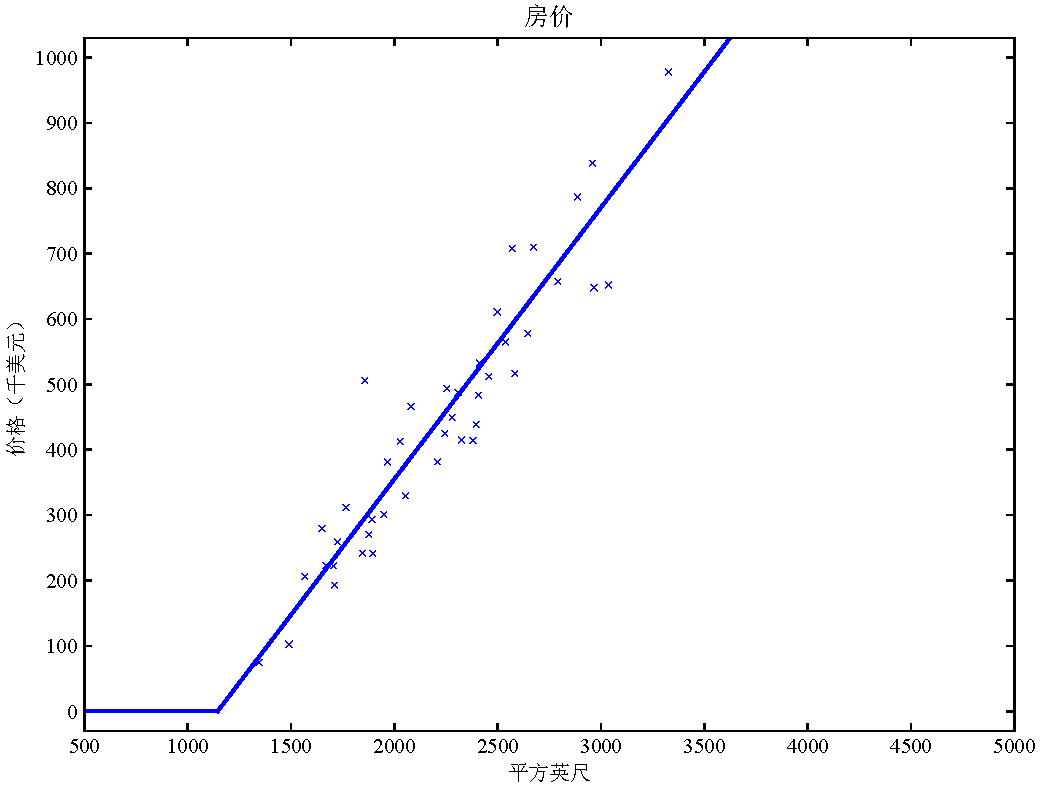
\includegraphics[width=0.5\linewidth]{figs/house_dataset_relu.pdf}
    \caption{带拐点的房价拟合}
    \label{fig:7.1}
\end{figure}

项 $b$ 通常被称为“偏置”,向量 $w$ 被称为权重向量。这样的神经网络称之为 1 层。(后续将定义多层的含义。)

\subsection*{堆叠神经元}

更复杂的神经网络可以将上述单个神经元“堆叠”在一起,使得一个神经元的输出作为下一个神经元的输入,从而产生更复杂的函数。
现在来深化房价预测的例子。除了房屋大小,假设还知道卧室数量、邮政编码和社区财富。构建神经网络类似于乐高积木:将单个积木堆叠在一起以构建复杂的结构。 这同样适用于神经网络:将单个神经元堆叠在一起以创建复杂的神经网络。
给定这些特征 (大小、卧室数量、邮政编码和财富),可能会决定房屋价格取决于其可容纳的最大家庭人数。假设家庭人数是房屋大小和卧室数量的函数 (参见图 \ref{fig:7.2})。邮政编码可以提供额外信息,例如社区的步行便利程度 (即,是否可以步行到杂货店或需要开车)。结合邮政编码和社区财富可以预测当地小学的质量。可以认为,房屋价格最终取决于这三个特征。

\begin{figure}[H]
\centering
\begin{tikzpicture}
\tikzstyle{nnnode}=[circle,draw,minimum size=1.5em]
    \node (phi2) [nnnode] {};
    \node (phi1) [nnnode, above=4mm of phi2] {};
    \node (phi3) [nnnode, below=6mm of phi2] {};
    \node (size) [above left=0mm and 5mm of phi1, label=left:{大小}] {};
    \node (bedrooms) [below left=0mm and 5mm of phi1, label=left:{卧室数量}] {};
    \node (zipcode) [below left=1mm and 5mm of phi2, label=left:{邮政编码}] {};
    \node (wealth) [below left=0mm and 5mm of phi3, label=left:{财富}] {};

    \node (output) [nnnode, right=25mm of phi2, label=right:{价格 $y$}] {};

    \draw[->] (phi1) -- (output) node [sloped, midway, yshift=7pt, font=\scriptsize] {家庭人数};
    \draw[->] (phi2) -- (output) node [sloped, near start, yshift=-7pt, font=\scriptsize] {\quad 步行便利程度};
    \draw[->] (phi3) -- (output) node [sloped, midway, yshift=-7pt, font=\scriptsize] {学校质量};
    \draw[->] (size) -- (phi1);
    \draw[->] (bedrooms) -- (phi1);
    \draw[->] (zipcode) -- (phi2);
    \draw[->] (zipcode) -- (phi3);
    \draw[->] (wealth) -- (phi3);
\end{tikzpicture}
\caption{预测房屋价格的小型神经网络示意图}\label{fig:7.2}
\end{figure}

形式上,神经网络的输入是一组输入特征 $x_1, x_2, x_3, x_4$。将“家庭人数”、“步行便利程度”和“学校质量”的中间变量记为 $a_1, a_2, a_3$ (这些 $a_i$ 通常被称为“隐藏单元”或“隐藏神经元”)。将每个 $a_i$ 表示为以 $x_1, \dots, x_4$ 的子集为输入的单神经元神经网络。然后,如在图 \ref{fig:7.1} 中,将有以下参数化:
\begin{align*}
    a_1 &= \text{ReLU}(\theta_1 x_1 + \theta_2 x_2 + \theta_3) \\
    a_2 &= \text{ReLU}(\theta_4 x_3 + \theta_5) \\
    a_3 &= \text{ReLU}(\theta_6 x_3 + \theta_7 x_4 + \theta_8)
\end{align*}
其中 $(\theta_1, \dots, \theta_8)$ 是参数。现在将最终输出 $\bar{h}_\theta(x)$ 表示为以 $a_1, a_2, a_3$ 为输入的另一个线性函数,得到\footnote{通常,对于多层神经网络,在末端,靠近输出处,不会应用 ReLU,特别是当输出不一定是正数时。}
\begin{equation}
    \bar{h}_\theta(x) = \theta_9 a_1 + \theta_{10} a_2 + \theta_{11} a_3 + \theta_{12}
    \label{eq:7.13}
\end{equation}
其中 $\theta$ 包含所有参数 $(\theta_1, \dots, \theta_{12})$。

现在将输出表示为以参数 $\theta$ 为输入的相当复杂的函数 $x$。然后可以使用第 \ref{sec:7.1} 节中的机制来学习参数 $\theta$。

\subsection*{生物神经网络的启发}

顾名思义,人工神经网络受到生物神经网络的启发。隐藏单元 $a_1, \dots, a_m$ 对应于生物神经网络中的神经元,参数 $\theta_i$ 对应于突触。然而,现代深度人工神经网络与生物神经网络的相似程度尚不清楚。例如,也许没有多少神经科学家认为生物神经网络可以有 1000 层,而一些现代人工神经网络则不然 (将在后续中详细阐述层的概念)。此外,人类大脑更新神经网络的方式是否与计算机科学家学习人工神经网络的方式 (使用反向传播,将在下一节介绍) 相似,这是一个悬而未决的问题。

\subsection*{两层全连接神经网络}

通过利用关于“家庭人数”、“步行便利程度”和“学校质量”如何由输入决定的重要先验知识/信念,构建了公式 \eqref{eq:7.13} 中的神经网络。隐含地假设知道家庭人数是一个重要的数量,并且它只能由“大小”和“卧室数量”确定。这样的先验知识可能不适用于其他应用。更灵活和通用的方法是为中间变量 $a_i$ 编写一个通用的参数化,作为所有 $x_1, \dots, x_4$ 的函数:
\begin{align}
    a_1 &= \text{ReLU}(w_1^\top x + b_1), \text{其中}\  w_1 \in \mathbb{R}^4 \text{且}\  b_1 \in \mathbb{R} \label{eq:7.14}\\
    a_2 &= \text{ReLU}(w_2^\top x + b_2), \text{其中}\  w_2 \in \mathbb{R}^4 \text{且}\  b_2 \in \mathbb{R} \notag\\
    a_3 &= \text{ReLU}(w_3^\top x + b_3), \text{其中}\  w_3 \in \mathbb{R}^4 \text{且}\  b_3 \in \mathbb{R} \notag
\end{align}

仍然使用上面定义的 $a_1, a_2, a_3$ 来定义 $\bar{h}_\theta(x)$。这样就得到了一个所谓的\textbf{全连接神经网络 (fully-connected neural network)},因为所有中间变量 $a_i$ 都依赖于所有输入 $x_i$。

为了通用性,具有 $m$ 个隐藏单元和 $d$ 维输入 $x \in \mathbb{R}^d$ 的两层全连接神经网络定义为
\begin{align}
    \forall j \in \{1, \dots, m\}, \quad z_j &= w_j^{[1]^\top} x + b_j^{[1]} \ \text{其中}\  w_j^{[1]} \in \mathbb{R}^d, b_j^{[1]} \in \mathbb{R} 
    \label{eq:7.15}\\
    a_j &= \text{ReLU}(z_j), \notag \\
    a &= [a_1, \dots, a_m]^\top \in \mathbb{R}^m \notag \\
    \bar{h}_\theta(x) &= w^{[2]^\top} a + b^{[2]} \text{其中}\  w^{[2]} \in \mathbb{R}^m, b^{[2]} \in \mathbb{R}
    \label{eq:7.16}
\end{align}

请注意,默认情况下,$\mathbb{R}^d$ 中的向量被视为列向量,特别是 $a$ 是一个分量为 $a_1, a_2, \dots, a_m$ 的列向量。索引 $^{[1]}$ 和 $^{[2]}$ 用于区分两组参数:$w_j^{[1]}$ (每个都是 $\mathbb{R}^d$ 中的向量) 和 $w^{[2]}$ (它是 $\mathbb{R}^m$ 中的向量)。稍后将更详细地讨论这些。

\subsection*{向量化}

在引入具有更多层和更复杂结构的神经网络之前,将使用更多的矩阵和向量符号简化神经网络的表达式。向量化的另一个重要动机是实现中的速度。为了有效地实现神经网络,在使用循环时必须小心。在代码中实现公式 \eqref{eq:7.15} 的最自然方法可能是使用 for 循环。在实践中,当输入和隐藏单元的维度很高时,使用循环会导致代码运行非常慢。利用 GPU 的并行性对于深度学习的发展至关重要。

这催生了向量化。向量化不是使用循环,而是利用矩阵代数和高度优化的数值线性代数库 (例如 BLAS) 来快速运行神经网络计算。在深度学习时代之前,for 循环可能足以处理较小的数据集,但现代深度网络和最先进的数据集使用 for 循环将不可行。

将下面的两层全连接神经网络向量化。将权重矩阵 $W^{[1]} \in \mathbb{R}^{m \times d}$ 定义为所有向量 $w_j^{[1]}$ 的串联,如下所示:
\begin{equation}
    W^{[1]} = \begin{bmatrix}
    & - w_1^{[1]^\top} - & \\
    & - w_2^{[1]^\top} - & \\
    & \vdots & \\
    & - w_m^{[1]^\top} - &
    \end{bmatrix} \in \mathbb{R}^{m \times d}
    \label{eq:7.17}
\end{equation}

现在根据矩阵向量乘法的定义,可以将 $z = [z_1, \dots, z_m]^\top \in \mathbb{R}^m$ 写为
\begin{equation}
    \underbrace{\begin{bmatrix}
    & z_1 & \\
    & \vdots & \\
    & z_m &
    \end{bmatrix}}_{z \in \mathbb{R}^{m \times 1}} = \underbrace{\begin{bmatrix}
    & - w_1^{[1]^\top} - & \\
    & - w_2^{[1]^\top} - & \\
    & \vdots & \\
    & - w_m^{[1]^\top} - &
    \end{bmatrix}}_{W^{[1]} \in \mathbb{R}^{m \times d}} \underbrace{\begin{bmatrix}
    & x_1 & \\
    & x_2 & \\
    & \vdots & \\
    & x_d &
    \end{bmatrix}}_{x \in \mathbb{R}^{d \times 1}} + \underbrace{\begin{bmatrix}
    & b_1^{[1]} & \\
    & b_2^{[1]} & \\
    & \vdots & \\
    & b_m^{[1]} &
    \end{bmatrix}}_{b^{[1]} \in \mathbb{R}^{m \times 1}}
    \label{eq:7.18}
\end{equation}
或者简明地写成
\begin{equation}
    z = W^{[1]} x + b^{[1]}
    \label{eq:7.19}
\end{equation}
再次强调,在本书中,根据先前建立的约定,$\mathbb{R}^d$ 中的向量自动视为列向量,并且可以看作是一个 $d \times 1$ 维矩阵。(注意,这与 numpy 不同,在 numpy 中,向量在广播中被视为行向量。)

根据 $z \in \mathbb{R}^m$ 计算激活 $a \in \mathbb{R}^m$ 涉及 ReLU 函数的逐元素应用,这可以高效地并行计算。重载 ReLU 以进行逐元素应用 (也就是说,对于向量 $t \in \mathbb{R}^d$,ReLU($t$) 是一个向量,使得 $\text{ReLU}(t)_i = \text{ReLU}(t_i)$),所以,我们有
\begin{equation}
    a = \text{ReLU}(z)
    \label{eq:7.20}
\end{equation}

类似地定义 $W^{[2]} = [w^{[2]}]^\top \in \mathbb{R}^{1 \times m}$。那么,公式 \eqref{eq:7.16} 中的模型可以概括为
\begin{align}
    a &= \text{ReLU}(W^{[1]} x + b^{[1]}) \notag \\
    \bar{h}_\theta(x) &= W^{[2]} a + b^{[2]}
    \label{eq:7.21}
\end{align}
其中 $\theta$ 由 $W^{[1]}, W^{[2]}$ (通常称为权重矩阵) 和 $b^{[1]}, b^{[2]}$ (称为偏置) 组成。$W^{[1]}, b^{[1]}$ 的集合称为第一层,$W^{[2]}, b^{[2]}$ 称为第二层。激活 $a$ 称为隐藏层。两层神经网络也称为单隐藏层神经网络。

\subsection*{多层全连接神经网络}

有了这种简洁的表示法,就可以堆叠更多层以获得更深的全连接神经网络。令 $r$ 为层数 (权重矩阵数)。令 $W^{[1]}, \dots, W^{[r]}, b^{[1]}, \dots, b^{[r]}$ 为所有层的权重矩阵和偏置。那么多层神经网络可以写成
\begin{align}
    a^{[1]} &= \text{ReLU}(W^{[1]} x + b^{[1]}) \notag\\
    a^{[2]} &= \text{ReLU}(W^{[2]} a^{[1]} + b^{[2]}) \notag\\
    \dots \notag\\
    a^{[r-1]} &= \text{ReLU}(W^{[r-1]} a^{[r-2]} + b^{[r-1]}) \notag\\
    \bar{h}_\theta(x) &= W^{[r]} a^{[r-1]} + b^{[r]}
    \label{eq:7.22}
\end{align}

注意到,为了使上述方程有意义,权重矩阵和偏置需要具有兼容的维度。如果 $a^{[k]}$ 的维度为 $m_k$,则权重矩阵 $W^{[k]}$ 的维度应为 $m_k \times m_{k-1}$,偏置 $b^{[k]} \in \mathbb{R}^{m_k}$。此外,$W^{[1]} \in \mathbb{R}^{m_1 \times d}$ 且 $W^{[r]} \in \mathbb{R}^{1 \times m_{r-1}}$。

网络中的神经元总数为 $m_1 + \dots + m_r$,该网络中的参数总数为 $(d+1)m_1 + (m_1+1)m_2 + \dots + (m_{r-1}+1)m_r$。

有时为了符号一致性,也记 $a^{[0]} = x$ 且 $a^{[r]} = \bar{h}_\theta(x)$。那么有简单的递归关系
\begin{equation}
    a^{[k]} = \text{ReLU}(W^{[k]} a^{[k-1]} + b^{[k]}), \forall k = 1, \dots, r-1
    \label{eq:7.23}
\end{equation}
注意,如果在公式 \eqref{eq:7.22} 中有一个额外的 ReLU,则对于 $k=r$ 这也成立,但人们通常喜欢使最后一层为线性层 (即没有 ReLU),这样可以得到负输出,并且更容易将最后一层解释为线性模型。(关于可解释性的更多内容请参见本节的“与核方法的联系”段落。)

\subsection*{其他激活函数}

激活函数 ReLU 可以被许多其他将 $\mathbb{R}$ 映射到 $\mathbb{R}$ 的非线性函数 $\sigma(\cdot)$ 替换,例如
\begin{align}
    \sigma(z) &= \frac{1}{1 + e^{-z}} \quad (\text{sigmoid}) \label{eq:7.24} \\
    \sigma(z) &= \frac{e^z - e^{-z}}{e^z + e^{-z}} \quad (\text{tanh}) \label{eq:7.25} \\
    \sigma(z) &= \max\{z, \gamma z\}, \gamma \in (0, 1) \quad (\text{leaky ReLU}) \label{eq:7.26} \\
    \sigma(z) &= \frac{z}{2} \left[1 + \text{erf}\left(\frac{z}{\sqrt{2}}\right)\right] \quad (\text{GELU}) \label{eq:7.27} \\
    \sigma(z) &= \frac{1}{\beta} \log(1 + \exp(\beta z)), \beta > 0 \quad (\text{Softplus}) \label{eq:7.28}
\end{align}

\begin{figure}[H]
    \centering
    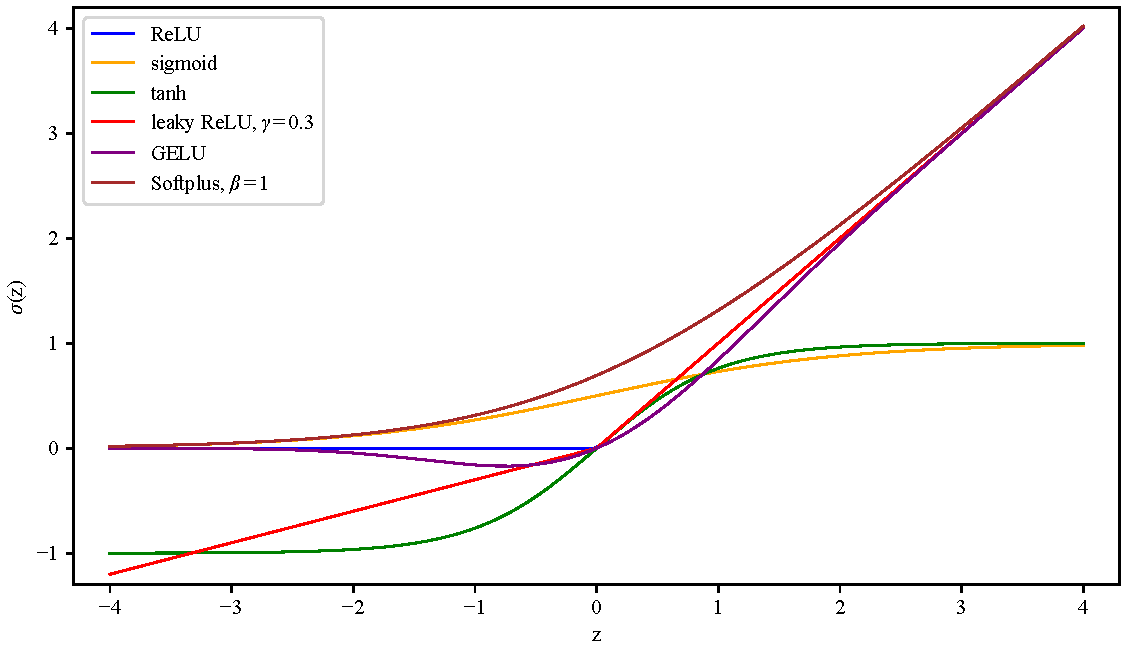
\includegraphics[width=0.8\linewidth]{figs/activations.pdf}
    \caption{深度学习中的激活函数}
    \label{fig:7.3}
\end{figure}

激活函数在图 \ref{fig:7.3} 中绘制。Sigmoid 和 tanh 现在使用得越来越少,部分原因是它们在两侧都有界,并且当 $z$ 趋于正负无穷时,它们的梯度会消失 (而所有其他激活函数在输入趋于正无穷时仍然有梯度)。Softplus 可以看作是 ReLU 的平滑版本,它具有适当的二阶导数,不过在实践中也不常用。GELU 和 leaky ReLU 都是 ReLU 的变体,但即使输入为负,它们也具有非零梯度。GELU (或其变体) 用于 NLP 模型,例如 BERT 和 GPT (这将在第 14 章讨论)。

\subsection*{为什么不使用恒等函数作为 $\sigma(z)$ ?} 

也即,为什么不使用 $\sigma(z) = z$?为了论证方便,假设 $b^{[1]}$ 和 $b^{[2]}$ 都为零。
假设 $\sigma(z) = z$,那么对于两层神经网络,有
\begin{align}
    \bar{h}_\theta(x) &= W^{[2]} a^{[1]} \label{eq:7.29} \\
    &= W^{[2]} \sigma(z^{[1]}) & \text{根据定义} \label{eq:7.30} \\
    &= W^{[2]} z^{[1]} & \text{因为}\  \sigma(z) = z \label{eq:7.31} \\
    &= W^{[2]} W^{[1]} x & \text{根据公式 \eqref{eq:7.18}} \label{eq:7.32} \\
    &= \tilde{W} x & \text{其中}\  \tilde{W} = W^{[2]} W^{[1]} \label{eq:7.33}
\end{align}
注意 $W^{[2]} W^{[1]}$ 如何合并成 $\tilde{W}$。

这是因为将一个线性函数应用于另一个线性函数会得到一个关于原始输入的线性函数 (即,可以构造一个 $\tilde{W}$ 使得 $\tilde{W} x = W^{[2]} W^{[1]} x$)。这会损失神经网络的许多表达能力,因为通常要预测的输出与输入之间存在非线性关系。如果没有非线性激活函数,神经网络将只会进行简单的线性回归。

\subsection*{与核方法的联系}

在之前的课程中,讨论了特征映射的概念。回忆一下,特征映射的主要动机是通过 $\theta^\top \phi(x)$ 来表示输入 $x$ 的非线性函数,其中 $\theta$ 是参数,$\phi(x)$ 是特征映射,是一个手工设计的关于原始输入 $x$ 的非线性函数。学习算法的性能很大程度上取决于特征映射 $\phi(x)$ 的选择。通常人们会利用领域知识来设计特征映射 $\phi(x)$ 以便适合特定的应用。选择特征映射的过程通常被称为\textbf{特征工程 (feature engineering)}。

可以将深度学习看作是一种自动学习正确特征映射(有时也称为“表示”)的方法,如下所示。假设用 $\beta$ 表示全连接神经网络(除了最后一层)的参数集合(公式 \eqref{eq:7.22})。然后可以将 $a^{[r-1]}$ 抽象为输入 $x$ 和参数 $\beta$ 的函数:$\beta: a^{[r-1]} = \phi_\beta(x)$。现在可以将模型写成
\begin{equation}
    \bar{h}_\theta(x) = W^{[r]} \phi_\beta(x) + b^{[r]} \label{eq:7.34}
\end{equation}
当 $\beta$ 固定时,$\phi_\beta(\cdot)$ 可以看作是特征映射,因此 $\bar{h}_\theta(x)$ 是关于特征 $\phi_\beta(x)$ 的线性模型。然而,训练神经网络时,参数 $\beta$ 和参数 $W^{[r]}, b^{[r]}$ 都会被优化,因此我们不仅在特征空间中学习线性模型,还在学习一个好的特征映射 $\phi_\beta(\cdot)$ 本身,以便在特征映射之上使用线性模型能够准确地进行预测。因此,深度学习倾向于较少依赖特定应用的领域知识,并且通常需要较少的特征工程。倒数第二层 $a^{[r]}$ 通常被(非正式地)称为深度学习背景下的学习特征或表示。

在房价预测的例子中,全连接神经网络不需要指定中间量,例如“家庭规模”,并且可以自动发现倒数第二层(即激活 $a^{[r-1]}$)中的一些有用特征,并使用它们来线性预测房价。从一个数据集获得的特征映射或表示(即函数 $\phi_\beta(\cdot)$)也可以用于其他数据集,这表明它们包含关于数据的基本信息。然而,通常神经网络会发现复杂的特征,这些特征对于预测输出非常有用,但对于人类来说可能难以理解或解释。这就是为什么有些人将神经网络称为\textit{黑箱 (black box)},因为很难理解它发现的特征。

\section{现代神经网络的模块}\label{sec:7.3}

第 \ref{sec:7.2} 节公式 \eqref{eq:7.22} 中介绍的多层神经网络现在通常被称为多层感知机 (MLP)。现代神经网络在实践中通常更复杂,由多个构建块或多层构建块组成。在本节中,将介绍一些其他的构建块并讨论可能的组合方式。

首先,每个矩阵乘法可以看作是一个构建块。考虑一个带有参数 $(W, b)$ 的矩阵乘法运算,其中 $W$ 是权重矩阵,$b$ 是偏置向量,作用于输入 $z$,
\begin{equation}
    \text{MM}_{W,b}(z) = W z + b. \label{eq:7.35}
\end{equation}
注意,这里隐含地假设所有维度都兼容。当在上下文中清晰或对讨论不重要时,也会省略 MM 的下标用以简化。

然后,MLP 可以写成多个矩阵乘法模块和非线性激活模块(也可以看作是构建块)的组合:
\begin{equation}
    \text{MLP}(x) = \text{MM}_{W^{[r]}, b^{[r]}} (\sigma(\text{MM}_{W^{[r-1]}, b^{[r-1]}} (\sigma(\cdots \text{MM}_{W^{[1]}, b^{[1]}}(x))))). \label{eq:7.36}
\end{equation}
或者,当省略表示参数的下标时,可以写成
\begin{equation}
    \text{MLP}(x) = \text{MM}(\sigma(\text{MM}(\sigma(\cdots \text{MM}(x))))). \label{eq:7.37}
\end{equation}
注意,在本讲义中,默认情况下,所有模块都有不同的参数集,并且参数的维度是有意义的。

较大的模块也可以通过较小的模块定义,例如,一个激活层 $\sigma$ 和一个矩阵乘法层 MM 经常组合在一起,在许多论文中被称为“层”。人们通常通过在图中指示这些模块之间的依赖关系来绘制架构。例如,参见图 \ref{fig:7.4} 左侧的 MLP 示意图。

\subsection*{残差连接}

一种非常有影响力的用于视觉应用的神经网络架构是 ResNet,它使用了残差连接,这些连接现在几乎用于所有大规模深度学习架构中。使用上面介绍的符号,一个非常简化的残差块可以定义为
\begin{equation}
    \text{Res}(z) = z + \sigma(\text{MM}(\sigma(\text{MM}(z)))). \label{eq:7.38}
\end{equation}
一个简化版 ResNet 是许多残差块的组合,后接一个矩阵乘法,
\begin{equation}
    \text{ResNet-S}(x) = \text{MM}(\text{Res}(\text{Res}(\cdots \text{Res}(x)))). \label{eq:7.39}
\end{equation}
这些模块的依赖关系也绘制在图 \ref{fig:7.4} 右侧。

\begin{figure}[H]
    \centering
    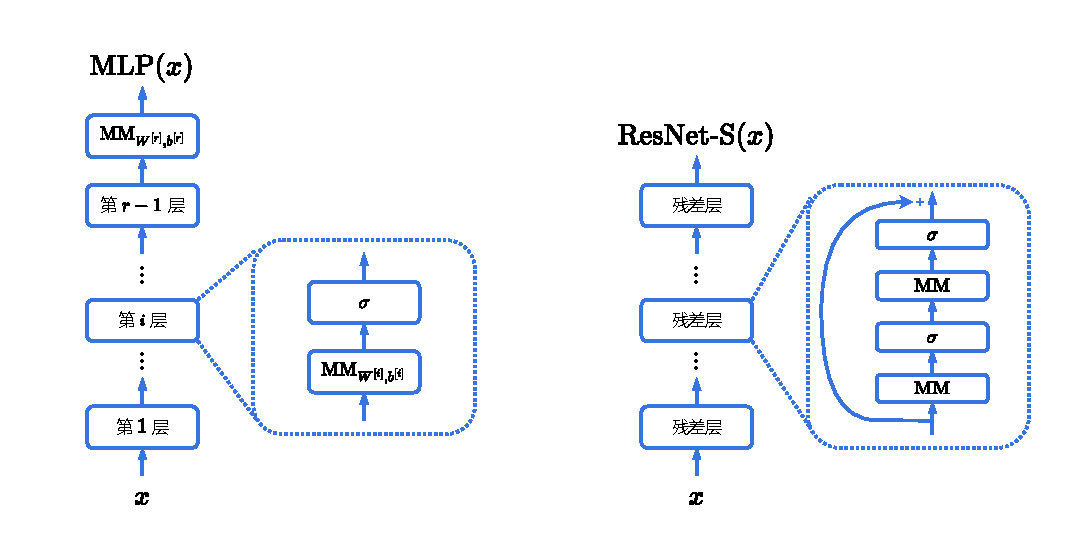
\includegraphics[width=1.0\linewidth]{figs/nn_architecture.pdf}
    \caption{网络架构示意图。\textbf{左图:} $r$ 层的MLP。\textbf{右图:} 残差网络。}
    \label{fig:7.4}
\end{figure}

注意,ResNet-S 与经典论文 [\cite{he2016resnet}] 中介绍的 ResNet 架构仍不完全相同,因为 ResNet 使用卷积层而不是普通的矩阵乘法,并在卷积和激活之间添加了批量归一化。下面将介绍卷积层和批量归一化的一些变体。ResNet-S 和层归一化是 Transformer 架构的一部分,它们在现代大型语言模型中被广泛使用。

\subsection*{层归一化}

层归一化,本文中记为 LN,是一个将向量 $z \in \mathbb{R}^m$ 映射到规范化的向量 $\text{LN}(z) \in \mathbb{R}^m$ 的模块。它通常在非线性激活之后使用。

首先定义层归一化的一个子模块,记为 LN-S。
\begin{equation}
    \text{LN-S}(z) = \begin{bmatrix}
        &\frac{z_1 - \hat{\mu}}{\hat{\sigma}}& \\
        &\frac{z_2 - \hat{\mu}}{\hat{\sigma}}& \\
        &\vdots& \\
        &\frac{z_m - \hat{\mu}}{\hat{\sigma}}&
    \end{bmatrix}, \label{eq:7.40}
\end{equation}
其中 $\hat{\mu} = \frac{\sum_{i=1}^m z_i}{m}$ 是向量 $z$ 的实际均值,$\hat{\sigma} = \sqrt{\frac{\sum_{i=1}^m (z_i - \hat{\mu})^2}{m}}$ 是 $z$ 中元素的实际标准差。\footnote{注意,这里的实际标准差是除以 $m$ 而不是 $m-1$,因为所感兴趣的是使 $\text{LN-S}(z)$ 的输出的平方和等于 1(与统计学中估计标准差不同)。} 直观上看,LN-S$(z)$ 是一个经过归一化处理的向量,其实际均值为零,实际标准差为 1。

通常零均值和标准差 1 并非最理想的归一化方案,因此层归一化引入了可学习的标量参数 $\beta$ 和 $\gamma$ 作为期望的均值和标准差,并使用仿射变换将 LN-S$(z)$ 的输出转换为均值为 $\beta$、标准差为 $\gamma$ 的向量。
\begin{equation}
    \text{LN}(z) = \beta + \gamma \cdot \text{LN-S}(z) = \begin{bmatrix}
        &\beta + \gamma \left(\frac{z_1 - \hat{\mu}}{\hat{\sigma}}\right)& \\
        &\beta + \gamma \left(\frac{z_2 - \hat{\mu}}{\hat{\sigma}}\right)& \\
        &\vdots& \\
        &\beta + \gamma \left(\frac{z_m - \hat{\mu}}{\hat{\sigma}}\right)&
    \end{bmatrix}. \label{eq:7.41}
\end{equation}
这里,第一个 $\beta$ 技术上应该解释为一个所有元素都是标量 $\beta$ 的向量。还需要注意,$\hat{\mu}$ 和 $\hat{\sigma}$ 也是 $z$ 的函数,在计算层归一化的导数时不应将其视为常数。此外,$\beta$ 和 $\gamma$ 是可学习参数,因此层归一化是一个带参数的模块(与不带任何参数的激活层不同)。

\vspace{0.5em}
\noindent\textit{尺度不变性:}层归一化一个重要的性质是它使得模型对参数的缩放具有不变性,具体如下。假设考虑将 LN 与 $\text{MM}_{W,b}(z)$ 组合,得到一个子网络 $\text{LN}(\text{MM}_{W,b}(z))$。那么,当 $\text{MM}_{W,b}$ 中的参数被缩放时,这个子网络的输出不会改变:
\begin{equation}
    \text{LN}(\text{MM}_{\alpha W, \alpha b}(z)) = \text{LN}(\text{MM}_{W,b}(z)), \forall \alpha > 0. \label{eq:7.42}
\end{equation}
为了说明这一点,首先知道 LN-S$(\cdot)$ 是尺度不变的:
\begin{equation}
    \text{LN-S}(\alpha z) = \begin{bmatrix}
        &\frac{\alpha z_1 - \alpha \hat{\mu}}{\alpha \hat{\sigma}}& \\
        &\frac{\alpha z_2 - \alpha \hat{\mu}}{\alpha \hat{\sigma}}& \\
        &\vdots& \\
        &\frac{\alpha z_m - \alpha \hat{\mu}}{\alpha \hat{\sigma}}&
    \end{bmatrix} = \begin{bmatrix}
        &\frac{z_1 - \hat{\mu}}{\hat{\sigma}}& \\
        &\frac{z_2 - \hat{\mu}}{\hat{\sigma}}& \\
        &\vdots& \\
        &\frac{z_m - \hat{\mu}}{\hat{\sigma}}&
    \end{bmatrix} = \text{LN-S}(z). \label{eq:7.43}
\end{equation}
然后有
\begin{align}
    \text{LN}(\text{MM}_{\alpha W, \alpha b}(z)) &= \beta + \gamma \text{LN-S}(\text{MM}_{\alpha W, \alpha b}(z)) \label{eq:7.44} \\
    &= \beta + \gamma \text{LN-S}(\alpha \text{MM}_{W,b}(z)) \label{eq:7.45} \\
    &= \beta + \gamma \text{LN-S}(\text{MM}_{W,b}(z)) \label{eq:7.46} \\
    &= \text{LN}(\text{MM}_{W,b}(z)). \label{eq:7.47}
\end{align}

由于这一性质,大多数用于大规模计算机视觉和语言应用的现代深度学习架构都具有以下尺度不变性,即对于除最后一层权重 $W_{\text{last}}$ 以外的所有权重 $W$,网络 $f$ 具有 $f_{W_{\text{last}}, \alpha W}(x) = f_{W_{\text{last}}, W}(x)$ 对于任意 $\alpha > 0$ 成立。这里,最后一层的权重是特殊的,因为在最后一层权重之后通常没有层归一化或批量归一化。

\vspace{0.5em}
\noindent\textit{其他归一化层:}还有几种其他归一化层,旨在将神经网络的中间层归一化到更固定和可控的尺度,例如批量归一化 [?] 和组归一化 [?]。批量归一化和组归一化更常用于计算机视觉应用,而层归一化更常用于语言应用。

\subsection*{卷积层}

卷积神经网络是由卷积层(以及许多其他模块)组成的神经网络,特别适用于计算机视觉应用。为了简化说明,本文重点介绍 1-D 卷积,并在本小节末尾非正式地简要提及 2-D 卷积。(2-D 卷积更适合于具有两个维度的图像。1-D 卷积也用于自然语言处理。)

首先介绍一个简化版本的 1-D 卷积层,记为 Conv1D-S$(\cdot)$,它是一种具有特殊结构的矩阵乘法层。Conv1D-S 的参数是一个滤波器向量 $w \in \mathbb{R}^k$,其中 $k$ 称为滤波器大小(通常 $k \ll m$),以及一个标量偏置 $b$。滤波器有时也称为核(但与核方法中的核无关)。为简单起见,假设 $k = 2\ell + 1$ 是一个奇数。首先在输入向量 $z$ 的两端填充零,即 $z_{1-\ell} = z_{1-\ell+1} = \cdots = z_0 = 0$ 和 $z_{m+1} = z_{m+2} = \cdots = z_{m+\ell} = 0$,并将 $z$ 看作一个 $(m+2\ell)$ 维向量。Conv1D-S 输出一个维度为 $\mathbb{R}^m$ 的向量,其中每个输出维度是 $z$ 中子集元素的线性组合,系数来自 $w$,
\begin{equation}
    \text{Conv1D-S}(z)_i = w_1 z_{i-\ell} + w_2 z_{i-\ell+1} + \cdots + w_{2\ell+1} z_{i+\ell} = \sum_{j=1}^{2\ell+1} w_j z_{i-\ell+(j-1)}. \label{eq:7.48}
\end{equation}
因此,可以将 Conv1D-S 视为具有共享参数的矩阵乘法:$\text{Conv1D-S}(z) = Qz$,其中
\begin{equation}
    Q = \begin{bmatrix}
        &w_{\ell+1} &\cdots &w_{2\ell+1} & &\\
        &\vdots     &\ddots &\ddots      &w_{2\ell+1} & &\\
        &w_1        &\ddots &\ddots      &\ddots &\ddots & &\\
        &           &w_1    &\ddots      &\ddots &\ddots &w_{2\ell+1} &\\
        &           &       &\ddots      &\ddots &\ddots &\vdots &\\
        &           &       &            &w_1    &\cdots &w_{\ell+1} &
        
    \end{bmatrix}. \label{eq:7.49}
\end{equation}
注意,$Q_{i,j} = Q_{i-1,j-1}$ 对于所有 $i, j \in \{2, \ldots, m\}$ 都成立,因此卷积是一种带有参数共享的矩阵乘法。还注意到,计算卷积只需要 $O(km)$ 的时间,而计算一般的矩阵乘法需要 $O(m^2)$ 的时间。卷积有 $k$ 个参数,而一般的矩阵乘法有 $m^2$ 个参数。因此,卷积应该比一般的矩阵乘法效率高得多(只要施加的附加结构不损害模型的灵活性以适应数据)。

还注意到,在实践中存在许多卷积层的变体,与这里定义的有所不同,例如,填充零的方式或有时卷积层输出的维度可能与输入的维度不同。为了简化,这里省略了一些这些细节。

实践中使用的卷积层也有许多“通道”,上面的简化版本对应于 1 通道版本。形式上,Conv1D 接受 $C$ 个向量 $z_1, \ldots, z_C \in \mathbb{R}^m$ 作为输入,其中 $C$ 称为通道数。换句话说,更一般的版本 Conv1D 接受一个矩阵作为输入,它是 $z_1, \ldots, z_C$ 的拼接,维度为 $m \times C$。它可以输出 $C'$ 个维度为 $m$ 的向量,记为 $\text{Conv1D}(z)_1, \ldots, \text{Conv1D}(z)_{C'}$,其中 $C'$ 称为输出通道,或等效地一个维度为 $m \times C'$ 的矩阵。每个输出是应用于不同通道的简化卷积之和。
\begin{equation}
    \forall i \in [C'], \text{Conv1D}(z)_i = \sum_{j=1}^C \text{Conv1D-S}_{i,j}(z_j). \label{eq:7.50}
\end{equation}
注意,每个 $\text{Conv1D-S}_{i,j}$ 都是具有不同参数的模块,因此总参数数量是 $k \times C \times C'$(Conv1D-S 的参数数量 $\times$ Conv1D-S$_{i,j}$ 的数量)$= kCC'$。相比之下,从 $\mathbb{R}^{m \times C}$ 到 $\mathbb{R}^{m \times C'}$ 的一般线性映射具有 $m^2CC'$ 个参数。卷积的参数也可以表示为维度为 $k \times C \times C'$ 的三维张量。

\vspace{0.5em}
\noindent\textit{2-D 卷积(简述):}单通道的 2-D 卷积,记为 Conv2D-S,类似于 Conv1D-S,但接受一个 2 维输入 $z \in \mathbb{R}^{m \times m}$ 并应用一个 $k \times k$ 大小的滤波器,输出 Conv2D-S$(z) \in \mathbb{R}^{m \times m}$。完整的 2-D 卷积层,记为 Conv2D,接受一系列矩阵 $z_1, \ldots, z_C \in \mathbb{R}^{m \times m}$ 作为输入,或者等效地一个 3-D 张量 $z = (z_1, \ldots, z_C) \in \mathbb{R}^{m \times m \times C}$,并输出一系列矩阵 $\text{Conv2D}(z)_1, \ldots, \text{Conv2D}(z)_{C'} \in \mathbb{R}^{m \times m}$,也可以看作一个维度为 $\mathbb{R}^{m \times m \times C'}$ 的 3D 张量。每个输出通道是应用于所有输入通道的 Conv2D-S 层结果的总和。
\begin{equation}
    \forall i \in [C'], \text{Conv2D}(z)_i = \sum_{j=1}^C \text{Conv2D-S}_{i,j}(z_j). \label{eq:7.51}
\end{equation}
因为有 $CC'$ 个 Conv2D-S 模块,并且每个 Conv2D-S 模块有 $k^2$ 个参数,所以总参数数量是 $CC'k^2$。其参数也可以看作一个维度为 $C \times C' \times k \times k$ 的四维张量。

\section{反向传播}\label{sec:7.4}

本节将介绍反向传播,或称自动微分,它能高效地计算损失函数的梯度 $\nabla J(\theta)$。首先,从一个非正式定理开始,该定理指出,只要一个\textit{实值函数 (real-valued function)} $f$ 可以通过一个可微网络或电路高效地计算/评估,那么它的梯度也可以在相似的时间内高效地计算。然后,将展示如何在神经网络中具体实现这一点。

由于通用定理的严格性并非本节的主要重点,将使用非正式定义来介绍术语。可微电路或可微网络是指一系列可微算术运算 (加法、减法、乘法、除法等) 和基本可微函数 (ReLU、exp、log、sin、cos 等) 的组合。电路的大小定义为这些运算和基本函数的总数。假设每个运算和函数及其导数或偏导数都可以在 $O(1)$ 时间内计算。

\begin{theorem}\label{theorem:7.4.1}
    \textit{[反向传播,或称自动微分的非正式表述]} 
    
    \noindent 假设有一个大小为 $N$ 的可微电路计算一个实值函数 $f: \mathbb{R}^\ell \to \mathbb{R}$。那么,梯度 $\nabla f$ 可以通过一个大小为 $O(N)$ 的电路在 $O(N)$ 的时间内计算。\footnote{注意到,如果函数 $f$ 的输出不依赖于某些输入的分量,则默认将关于这些分量的梯度设为零。在本节的计算方案中,将梯度设为零不计入总运行时间。因此,当 $N \le \ell$ 时,可以在 $O(N)$ 时间内计算梯度,这可能甚至小于 $\ell$。}
\end{theorem}

注意到,对于第 $j$ 个样本的损失函数 $J^{(j)}(\theta)$ 可以通过包含加法、减法、乘法和非线性激活等运算和函数的序列计算。因此,定理表明,应该能够在与计算 $J^{(j)}(\theta)$ 本身相似的时间内计算 $\nabla J^{(j)}(\theta)$。这不仅适用于第 \ref{sec:7.2} 节介绍的全连接神经网络,也适用于许多其他使用更高级模块的神经网络。

注意到,自动微分或反向传播已经集成到所有深度学习库中,例如 tensorflow 和 pytorch,因此在实践中,大多数情况下研究人员无需编写自己的反向传播算法。然而,理解其原理对于深入理解深度学习的工作原理非常有帮助。

本节的其余部分组织如下。在第 \ref{sec:7.4.1} 节中,将从一个新的角度回顾基本链式法则,这对于理解反向传播特别有用。第 \ref{sec:7.4.2} 节将介绍反向传播的通用策略。第 \ref{sec:7.4.2} 节将讨论如何计算神经网络中使用的基本模块的所谓反向函数,第 \ref{sec:7.4.4} 节将把所有内容组合起来,得到一个用于 MLP 的具体反向传播算法。

\subsection{偏导数初步}\label{sec:7.4.1}

假设标量变量 $J$ 依赖于某些变量 $z$ (可以是标量、矩阵或高阶张量),记 $\frac{\partial J}{\partial z}$ 为 $J$ 关于变量 $z$ 的偏导数。这里的惯例是 $\frac{\partial J}{\partial z}$ 与 $z$ 本身具有完全相同的维度。例如,如果 $z \in \mathbb{R}^{m \times n}$,则 $\frac{\partial J}{\partial z} \in \mathbb{R}^{m \times n}$,并且 $\frac{\partial J}{\partial z}$ 的 $(i, j)$ 元素等于 $\frac{\partial J}{\partial z_{ij}}$。

\begin{remark}\label{remark:7.4.1}
    当 $J$ 和 $z$ 都不是标量时,$J$ 关于 $z$ 的偏导数变成矩阵或张量,并且符号变得有些棘手。除了处理数学或符号上的挑战之外,这些多元函数的偏导数不仅计算和存储成本高昂,而且实际上也很少显式构造这些偏导数。作者的经验表明,只考虑标量函数对向量、矩阵或张量的导数通常更有效。故在本讲义中,不会讨论多元函数的导数。
\end{remark} 

\subsubsection*{链式法则}

下面回顾微积分中的链式法则,但我们的视角和符号更侧重于自动微分。

考虑一个标量变量 $J$,它由函数 $f$ 和 $g$ 在某个变量 $z$ 上的复合得到,
\begin{align}
    z &\in \mathbb{R}^m \notag\\
    u &= g(z) \in \mathbb{R}^n \notag\\
    J &= f(u) \in \mathbb{R}. \label{eq:7.52}
\end{align}
下面的推导可以很容易地扩展到 $z$ 和 $u$ 是矩阵或张量的情况;但需要强调的是,最终变量 $J$ 是一个标量(参见备注 \ref{remark:7.4.1})。令 $u = (u_1, \dots, u_n)$,并令 $g(z) = \left(g_1(z), \dots, g_n(z)\right)$。那么,根据标准的链式法则,有
\begin{equation}
    \forall i \in \{1, \dots, m\}, \quad \frac{\partial J}{\partial z_i} = \sum_{j=1}^n \frac{\partial J}{\partial u_j} \cdot \frac{\partial g_j}{\partial z_i}. \label{eq:7.53}
\end{equation}
或者,当 $z$ 和 $u$ 都是向量时,采用向量化符号:
\begin{equation}
    \frac{\partial J}{\partial z} = \begin{bmatrix}
    &\frac{\partial g_1}{\partial z_1}&  &\cdots&  &\frac{\partial g_n}{\partial z_1}& \\
    &\vdots&  &\ddots&  &\vdots& \\
    &\frac{\partial g_1}{\partial z_m}&  &\cdots&  &\frac{\partial g_n}{\partial z_m}&
    \end{bmatrix} \cdot \frac{\partial J}{\partial u}. \label{eq:7.54}
\end{equation}
换句话说,反向函数总是从 $\frac{\partial J}{\partial u}$ 到 $\frac{\partial J}{\partial z}$ 的线性映射,但请注意,映射本身可以以复杂的方式依赖于 $z$。公式 \eqref{eq:7.54} 右侧的矩阵实际上是函数 $g$ 的雅可比矩阵的转置。然而,不会深入讨论雅可比矩阵的应用,以避免复杂性。部分原因在于,当 $z$ 是矩阵(或张量)时,要写出类似公式 \eqref{eq:7.54} 的形式,需要将 $z$ 展平为向量或引入张量-矩阵乘法的额外符号。从这个意义上说,公式 \eqref{eq:7.53} 在所有情况下都更方便有效。例如,当 $z \in \mathbb{R}^{r \times s}$ 是一个矩阵时,可以很容易地重写公式 \eqref{eq:7.53} 得到
\begin{equation}
    \forall i, k, \quad \frac{\partial J}{\partial z_{ik}} = \sum_{j=1}^n \frac{\partial J}{\partial u_j} \cdot \frac{\partial g_j}{\partial z_{ik}}, \label{eq:7.55}
\end{equation}
这将在第 \ref{sec:7.4.3} 节的一些推导中用到。

\vspace{0.5em}
\noindent\textit{链式法则的关键解释:}可以将上面的公式(公式 \eqref{eq:7.53} 或 \eqref{eq:7.54})看作是从 $\frac{\partial J}{\partial u}$ 计算 $\frac{\partial J}{\partial z}$ 的一种方法。考虑以下抽象问题:假设 $J$ 通过公式 \eqref{eq:7.52} 中定义的 $u$ 依赖于 $z$。然而,假设函数 $f$ 未知或函数 $f$ 很复杂,但已知 $\frac{\partial J}{\partial u}$ 的值。那么,公式 \eqref{eq:7.54} 提供了一种从 $\frac{\partial J}{\partial u}$ 计算 $\frac{\partial J}{\partial z}$ 的方法。
\begin{equation}
    \frac{\partial J}{\partial u} \quad \xRightarrow[\text{只需要关于}\  g(\cdot) \ \text{和}\  z \text{的信息}]{\text{利用链式法则和公式 \eqref{eq:7.54}} } \quad \frac{\partial J}{\partial z}. \label{eq:7.56}
\end{equation}
此外,此公式仅涉及关于 $g$ 的知识(更准确地说,$\frac{\partial g_j}{\partial z_i}$)。将反复利用这一点来处理 $g$ 是复杂网络 $f$ 的构建模块的情况。

根据经验,可以将公式 \eqref{eq:7.53} 或 \eqref{eq:7.54} 中的映射模块视为一个黑盒,并且定义一个数学符号也便于后续讨论。\footnote{该函数也是 pytorch 中模块的\ .backward() 方法。} 使用 $\mathcal{B}[g, z]$ 定义将 $\frac{\partial J}{\partial u}$ 映射到 $\frac{\partial J}{\partial z}$ 的函数,并记作
\begin{equation}
    \frac{\partial J}{\partial z} = \mathcal{B}[g, z]\left(\frac{\partial J}{\partial u}\right). \label{eq:7.57}
\end{equation}
称 $\mathcal{B}[g, z]$ 为模块 $g$ 的\textbf{反向函数 (backward function)}。注意,当 $z$ 固定时,$\mathcal{B}[g, z]$ 仅是从 $\mathbb{R}^n$ 到 $\mathbb{R}^m$ 的线性映射。使用公式 \eqref{eq:7.53},有
\begin{equation}
    (\mathcal{B}[g, z](v))_i = \sum_{j=1}^m \frac{\partial g_j}{\partial z_i} \cdot v_j. \label{eq:7.58}
\end{equation}
或者采用向量化符号,使用公式 \eqref{eq:7.54},有
\begin{equation}
    \mathcal{B}[g, z](v) = \begin{bmatrix}
    &\frac{\partial g_1}{\partial z_1}&  &\cdots&  &\frac{\partial g_n}{\partial z_1}& \\
    &\vdots&  &\ddots&  &\vdots& \\
    &\frac{\partial g_1}{\partial z_m}&  &\cdots&  &\frac{\partial g_n}{\partial z_m}&
    \end{bmatrix} \cdot v. \label{eq:7.59}
\end{equation}
因此 $\mathcal{B}[g, z]$ 可以看作一个矩阵。然而,实际上,$z$ 将不断变化,因此当 $g$ 固定时,反向映射必须针对不同的 $z$ 重新计算。因此,从经验上看,反向函数 $\mathcal{B}[g, z](v)$ 通常被视为一个函数,它接受 $z$($g$ 的输入)和 $v$($J$ 对某个变量的梯度,该变量被认为是 $g$ 的输出)作为输入,并输出一个向量,该向量被认为是 $J$ 对 $z$ 的梯度。

\subsection{反向传播的通用策略}\label{sec:7.4.2}

本节讨论自动微分的通用策略,以建立高层次的理解。然后,将把这种方法实例化到具体的神经网络中。采用的观点是,神经网络是由小的构建块组成的复杂组合,例如第 \ref{sec:7.3} 节中定义的 MM、$\sigma$、Conv2D、LN 等。注意,损失函数(例如,均方误差损失或交叉熵损失)也可以抽象地视为附加模块。因此,可以将损失函数 $J$(针对单个样本 $(x, y)$)抽象地写成许多模块的组合:\footnote{严格来说,应该写成 $J = M_k(M_{k-1}(\cdots M_1(x)), y)$。然而,为了计算相对于参数的导数,将 $y$ 视为常数,因此为了符号的简洁性,可以将其视为 $M_k$ 的一部分。}
\begin{equation}
    J = M_k(M_{k-1}(\cdots M_1(x))). \label{eq:7.60}
\end{equation}

例如,对于具有 MLP $\bar{h}_\theta(x)$(在公式 \eqref{eq:7.36} 和 \eqref{eq:7.37} 中定义)的二分类问题,损失函数可以写成公式 \eqref{eq:7.60} 的形式,其中 $M_1 = \text{MM}_{W^{[1]}, b^{[1]}}$,$M_2 = \sigma$, $M_3 = \text{MM}_{W^{[2]}, b^{[2]}}$,$\dots$,以及 $M_{k-1} = \text{MM}_{W^{[r]}, b^{[r]}}$, $M_k = \ell_{\text{logistic}}$。

从这个例子可以看出,有些模块涉及参数,而有些模块可能只涉及固定的操作集。为了通用性,假设每个 $M_i$ 都涉及一组参数 $\theta^{[i]}$,尽管当 $M_i$ 是像非线性激活这样的固定操作时,$\theta^{[i]}$ 可能是一个空集。之后将更详细地讨论模块化的粒度,但目前假设所有模块 $M_i$ 都足够简单。

引入用于公式 \eqref{eq:7.60} 中计算的中间变量:
\begin{align}
    u^{[0]} &= x \notag\\
    u^{[1]} &= M_1(u^{[0]}) \notag\\
    u^{[2]} &= M_2(u^{[1]}) \notag\\
    &\vdots \notag\\
    J = u^{[k]} &= M_k(u^{[k-1]}). \tag{F}\label{eq:F}
\end{align}

反向传播由两个过程组成:前向传播和反向传播。在前向传播中,算法根据定义 \eqref{eq:F} 按顺序计算 $u^{[1]}, \dots, u^{[k]}$,并将所有中间变量 $u^{[i]}$ 保存在内存中。

在反向传播中,首先按反向顺序计算 $J$ 对中间变量的导数,即 $\frac{\partial J}{\partial u^{[k]}}, \dots, \frac{\partial J}{\partial u^{[1]}}$,然后从 $\frac{\partial J}{\partial u^{[i]}}$ 和 $u^{[i-1]}$ 计算参数 $\theta^{[i]}$ 的导数 $\frac{\partial J}{\partial \theta^{[i]}}$。这两类计算可以相互交织,因为 $\frac{\partial J}{\partial \theta^{[i]}}$ 仅依赖于 $\frac{\partial J}{\partial u^{[i]}}$ 和 $u^{[i-1]}$,而不依赖于任何 $k < i$ 的 $\frac{\partial J}{\partial u^{[k]}}$。

首先通过引用第 \ref{sec:7.4.1} 节关于链式法则的讨论来理解为什么 $\frac{\partial J}{\partial u^{[i-1]}}$ 可以从 $\frac{\partial J}{\partial u^{[i]}}$ 和 $u^{[i-1]}$ 有效计算。通过设置 $u = u^{[i]}$ 和 $z = u^{[i-1]}$,以及 $f(u) = M_k(M_{k-1}(\cdots M_{i+1}(u)))$,以及 $g(\cdot) = M_i(\cdot)$,来实例化讨论。注意,$f$ 非常复杂,但不需要关于 $f$ 的任何具体信息。那么,结论性公式 \eqref{eq:7.56} 对应于
\begin{equation}
    \frac{\partial J}{\partial u^{[i]}} \quad \xRightarrow[\textbf{只需要关于}\  M_i(\cdot) \ \textbf{和}\  u^{[i-1]} \ \textbf{的信息}]{\text{链式法则}} \frac{\partial J}{\partial u^{[i-1]}}. \label{eq:7.61}
\end{equation}
更准确地说,根据公式 \eqref{eq:7.57},可以写成
\begin{align}
    \frac{\partial J}{\partial u^{[i-1]}} &= \mathcal{B}[M_i, u^{[i-1]}]\left(\frac{\partial J}{\partial u^{[i]}}\right). \tag{B1}\label{eq:B1}
\end{align}
将链式法则实例化为 $z = \theta^{[i]}$ 和 $u = u^{[i]}$,也有
\begin{align}
    \frac{\partial J}{\partial \theta^{[i]}} &= \mathcal{B}[M_i, \theta^{[i]}]\left(\frac{\partial J}{\partial u^{[i]}}\right). \tag{B2}\label{eq:B2}
\end{align}
有关算法的说明,请参见图 \ref{fig:7.5}。

\begin{figure}[H]
    \centering
    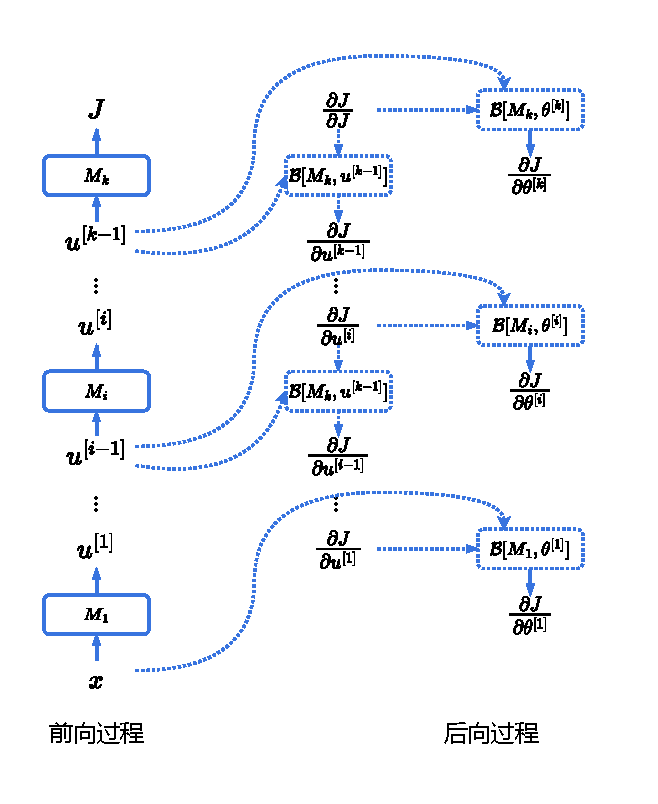
\includegraphics[width=0.7\linewidth]{figs/backpropagation.pdf}
    \caption{反向传播}
    \label{fig:7.5}
\end{figure}

\newpage
\begin{remark}\upshape
    \text{[计算效率和模块的粒度]} 
    
    \noindent 将复杂网络视为小型模块组合的主要根本目的是,小型模块往往具有可高效实现的后向函数。实际上,所有原子模块(如加法、乘法和 ReLU)的后向函数都可以像评估这些模块一样高效地计算(最多相差一个乘法常数因子)。利用这一事实,可以通过将神经网络视为许多原子操作的组合,并调用上面讨论的反向传播来证明定理 \ref{theorem:7.4.1}。然而,在实践中,会更常使用矩阵乘法、层归一化这类模块来模块化网络。正如后文所述,这些操作的后向函数的朴素实现也具有与这些函数的评估相同的运行时间。
\end{remark}


\subsection{基本模块的后向函数}\label{sec:7.4.3}

利用第 \ref{sec:7.4.2} 节的通用策略,只需计算网络中使用的所有模块 $M_i$ 的后向函数即可。本节计算基本模块 MM、激活函数 $\sigma$ 和损失函数的后向函数。

\vspace{0.5em}
\noindent\textit{MM 的后向函数:} 假设 $\text{MM}_{W,b}(z) = Wz + b$ 是一个矩阵乘法模块,其中 $z \in \mathbb{R}^m$ 且 $W \in \mathbb{R}^{n \times m}$。那么,对于 $v \in \mathbb{R}^n$,使用公式 \eqref{eq:7.59},有
\begin{equation}
    \mathcal{B}[\text{MM}, z](v) = \begin{bmatrix}
        &\frac{\partial (Wz+b)_1}{\partial z_1}& \cdots& \frac{\partial (Wz+b)_n}{\partial z_1}& \\
        &\vdots& \ddots& \vdots& \\
        &\frac{\partial (Wz+b)_1}{\partial z_m}& \cdots& \frac{\partial (Wz+b)_n}{\partial z_m}&
    \end{bmatrix} v. \label{eq:7.62}
\end{equation}
由于对于所有 $i \in [m], j \in [n]$,$\frac{\partial (Wz+b)_j}{\partial z_i} = \frac{\partial b_j + \sum_{k=1}^m W_{jk} z_k}{\partial z_i} = W_{ji}$,因此有
\begin{equation}
    \mathcal{B}[\text{MM}, z](v) = W^\top v \in \mathbb{R}^m. \label{eq:7.63}
\end{equation}
在上述推导中,将 MM 视为 $z$ 的函数。如果将 MM 视为 $W$ 和 $b$ 的函数,那么也可以计算参数变量 $W$ 和 $b$ 的后向函数。使用公式 \eqref{eq:7.59} 不太方便,因为变量 $W$ 是一个矩阵,而公式 \eqref{eq:7.59} 中的矩阵将是一个四阶张量,有书写难度。因此,使用 \eqref{eq:7.58}:
\begin{equation}
    (\mathcal{B}[\text{MM}, W](v))_{ij} = \sum_{k=1}^m \frac{\partial (Wz+b)_k}{\partial W_{ij}} \cdot v_k = \sum_{k=1}^m \frac{\partial \sum_{s=1}^m W_{ks} z_s}{\partial W_{ij}} \cdot v_k = v_i z_j. \label{eq:7.64}
\end{equation}
在向量化表示中,有
\begin{equation}
    \mathcal{B}[\text{MM}, W](v) = v z^\top \in \mathbb{R}^{n \times m}. \label{eq:7.65}
\end{equation}
对于变量 $b$,使用公式 \eqref{eq:7.59},有
\begin{equation}
    \mathcal{B}[\text{MM}, b](v) = \begin{bmatrix}
        &\frac{\partial (Wz+b)_1}{\partial b_1}& \cdots& \frac{\partial (Wz+b)_n}{\partial b_1}& \\
        &\vdots& \ddots& \vdots& \\
        &\frac{\partial (Wz+b)_1}{\partial b_n}& \cdots& \frac{\partial (Wz+b)_n}{\partial b_n}&
    \end{bmatrix} v = v. \label{eq:7.66}
\end{equation}
这里利用了当 $i \neq j$ 时 $\frac{\partial (Wz+b)_i}{\partial b_j} = 0$,当 $i = j$ 时 $\frac{\partial (Wz+b)_j}{\partial b_i} = 1$。

计算后向函数的计算效率是 $O(mn)$,与计算矩阵乘法结果的效率相同(相差一个常数因子)。

\vspace{0.5em}
\noindent\textit{激活函数的后向函数。} 假设 $M(z) = \sigma(z)$,其中 $\sigma$ 是一个逐元素的激活函数,且 $z \in \mathbb{R}^m$。那么,使用公式 \eqref{eq:7.59},有
\begin{align}
    \mathcal{B}[\sigma, z](v) &= \begin{bmatrix}
        &\frac{\partial \sigma(z_1)}{\partial z_1}& \cdots& \frac{\partial \sigma(z_m)}{\partial z_1}& \\
        &\vdots& \ddots& \vdots& \\
        &\frac{\partial \sigma(z_1)}{\partial z_m}& \cdots& \frac{\partial \sigma(z_m)}{\partial z_m}&
    \end{bmatrix} v \label{eq:7.67} \\
    &= \text{diag}(\sigma'(z_1), \dots, \sigma'(z_m))v \label{eq:7.68} \\
    &= \sigma'(z) \odot v \in \mathbb{R}^m. \label{eq:7.69}
\end{align}
这里利用了当 $j \neq i$ 时 $\frac{\partial \sigma(z_j)}{\partial z_i} = 0$,$\text{diag}(\lambda_1, \dots, \lambda_m)$ 表示对角线上为 $\lambda_1, \dots, \lambda_m$ 的对角矩阵,$\odot$ 表示两个同维度向量的逐元素乘积,$\sigma'(\cdot)$ 是激活函数 $\sigma$ 的导数(对向量逐元素应用)。关于计算效率,注意到乍一看,公式 \eqref{eq:7.67} 似乎表明后向函数需要 $O(m^2)$ 的时间,但公式 \eqref{eq:7.69} 表明它可以在 $O(m)$ 的时间内实现(这与评估函数的时间相同)。如果使用更小的模块,即把向量到向量的非线性激活视为 $m$ 个标量到标量的非线性激活,那么公式 \eqref{eq:7.67} 到 \eqref{eq:7.69} 的简化可能性不应感到惊讶,这时后向传播应该具有与前向传播相似的时间。

\vspace{0.5em}
\noindent\textit{损失函数的后向函数。} 当模块 $M$ 接受一个向量 $z$ 并输出一个标量时,根据公式 \eqref{eq:7.59},后向函数接受一个标量 $v$ 并输出一个向量,其分量为 $(\mathcal{B}[M, z](v))_i = \frac{\partial M}{\partial z_i} v$。因此,在向量化表示中,$\mathcal{B}[M, z](v) = \frac{\partial M}{\partial z} \cdot v$。

回想一下,平方损失 $\ell_{\text{MSE}}(z, y) = \frac{1}{2}(z-y)^2$。因此,$\mathcal{B}[\ell_{\text{MSE}}, z](v) = \frac{\partial \frac{1}{2}(z-y)^2}{\partial z} \cdot v = (z-y) \cdot v$。

对于逻辑损失,根据公式 \eqref{eq:2.6},有
\begin{equation}
    \mathcal{B}[\ell_{\text{logistic}}, t](v) = \frac{\partial \ell_{\text{logistic}}(t, y)}{\partial t} \cdot v = (1/(1 + \exp(-t)) - y) \cdot v. \label{eq:7.70}
\end{equation}

对于交叉熵损失,根据公式 \eqref{eq:2.17},有
\begin{equation}
    \mathcal{B}[\ell_{\text{ce}}, t](v) = \frac{\partial \ell_{\text{ce}}(t, y)}{\partial t} \cdot v = (\phi - e_y) \cdot v, \label{eq:7.71}
\end{equation}
其中 $\phi = \text{softmax}(t)$。

\subsection{MLP 的反向传播}\label{sec:7.4.4}

给定评估 MLP 损失所需的每个模块的后向函数,根据第 \ref{sec:7.4.2} 节的策略计算损失相对于隐藏激活和参数的梯度。
考虑一个具有逻辑损失的 $r$ 层 MLP。损失函数可以通过一系列操作计算(即前向传播),
\begin{align}
    z^{[1]} &= \text{MM}_{W^{[1]}, b^{[1]}}(x), \nonumber \\
    a^{[1]} &= \sigma(z^{[1]}), \nonumber \\
    z^{[2]} &= \text{MM}_{W^{[2]}, b^{[2]}}(a^{[1]}), \nonumber \\
    a^{[2]} &= \sigma(z^{[2]}), \nonumber \\
    &\vdots \nonumber \\
    z^{[r]} &= \text{MM}_{W^{[r]}, b^{[r]}}(a^{[r-1]}), \nonumber \\
    J &= \ell_{\text{logistic}}(z^{[r]}, y). \label{eq:7.72}
\end{align}
按后向顺序依次应用后向函数。首先,有
\begin{equation}
    \frac{\partial J}{\partial z^{[r]}} = \mathcal{B}[\ell_{\text{logistic}}, z^{[r]}]\left(\frac{\partial J}{\partial J}\right) = \mathcal{B}[\ell_{\text{logistic}}, z^{[r]}](1). \label{eq:7.73}
\end{equation}
然后,通过重复调用链式法则(公式 \eqref{eq:7.58}),迭代计算 $\frac{\partial J}{\partial a^{[i]}}$ 和 $\frac{\partial J}{\partial z^{[i]}}$:
\begin{align}
    \frac{\partial J}{\partial a^{[r-1]}} &= \mathcal{B}[\text{MM}, a^{[r-1]}]\left(\frac{\partial J}{\partial z^{[r]}}\right) \nonumber \\
    \frac{\partial J}{\partial z^{[r-1]}} &= \mathcal{B}[\sigma, z^{[r-1]}]\left(\frac{\partial J}{\partial a^{[r-1]}}\right) \nonumber \\
    &\vdots \nonumber \\
    \frac{\partial J}{\partial z^{[1]}} &= \mathcal{B}[\sigma, z^{[1]}]\left(\frac{\partial J}{\partial a^{[1]}}\right). \label{eq:7.74}
\end{align}
数值上,通过重复调用公式 \eqref{eq:7.69} 和 \eqref{eq:7.63},并选择不同的变量,计算这些量。
注意到中间值 $a^{[i]}$ 和 $z^{[i]}$ 在反向传播(公式 \eqref{eq:7.74})中使用,因此这些值需要在前向传播后存储在内存中。

接下来,通过调用公式 \eqref{eq:7.65} 和 \eqref{eq:7.66},计算参数的梯度:
\begin{equation}
    \begin{aligned}
        \frac{\partial J}{\partial W^{[r]}} &= \mathcal{B}[\text{MM}, W^{[r]}]\left(\frac{\partial J}{\partial z^{[r]}}\right) \\
        \frac{\partial J}{\partial b^{[r]}} &= \mathcal{B}[\text{MM}, b^{[r]}]\left(\frac{\partial J}{\partial z^{[r]}}\right) \\
        &\vdots \\
        \frac{\partial J}{\partial W^{[1]}} &= \mathcal{B}[\text{MM}, W^{[1]}]\left(\frac{\partial J}{\partial z^{[1]}}\right) \\
        \frac{\partial J}{\partial b^{[1]}} &= \mathcal{B}[\text{MM}, b^{[1]}]\left(\frac{\partial J}{\partial z^{[1]}}\right).
    \end{aligned} \label{eq:7.75}
\end{equation}

还注意到,公式 \eqref{eq:7.75} 中的计算块可以与公式 \eqref{eq:7.74} 中的计算块交织进行,因为一旦计算出 $\frac{\partial J}{\partial z^{[i]}}$,就可以计算出 $\frac{\partial J}{\partial W^{[i]}}$ 和 $\frac{\partial J}{\partial b^{[i]}}$。

将所有这些放在一起,并调用公式 \eqref{eq:7.72}、\eqref{eq:7.74} 和 \eqref{eq:7.75},得到以下算法(算法 \ref{algo:3}):

\vspace{0.5em}
\begin{algorithm}[H]\label{algo:3}
    \SetAlgoNoLine
    \caption{多层神经网络的反向传播算法}
    \textbf{前向过程:} 使用公式 \eqref{eq:7.72} 计算出 $a^{[k]}$, $z^{[k]}$, and $J$ 的值并存储下来。\\
    \textbf{反向过程:} 计算 $J$ 相对于 $z^{[r]}$ 的梯度:
    \begin{align}\label{eq:7.76}
        \frac{\partial J}{\partial z^{[r]}} &= \mathcal{B}[\ell_{\text{logistic}}, z^{[r]}] (1) = (1/(1 + \exp(-z^{[r]})) - y).
    \end{align}\\
    \For{$k = r-1$ \KwTo $0$}{
        计算相对于参数 $W^{[k+1]}$ 和 $b^{[k+1]}$ 的梯度:
        \begin{align}
            \frac{\partial J}{\partial W^{[k+1]}} &= \mathcal{B}[\text{MM}, W^{[k+1]}] \left( \frac{\partial J}{\partial z^{[k+1]}} \right) \nonumber \\
            &= \frac{\partial J}{\partial z^{[k+1]}} a^{[k]\top}. \label{eq:7.77}\\
            \frac{\partial J}{\partial b^{[k+1]}} &= \mathcal{B}[\text{MM}, b^{[k+1]}] \left( \frac{\partial J}{\partial z^{[k+1]}} \right) \nonumber \\
        &= \frac{\partial J}{\partial z^{[k+1]}}. \label{eq:7.78}
        \end{align}\\
        若 $k \ge 1$, 计算相对于 $z^{[k]}$ 和 $a^{[k]}$ 的梯度:
        \begin{align}
            \frac{\partial J}{\partial a^{[k]}} &= \mathcal{B}[\sigma, a^{[k]}] \left( \frac{\partial J}{\partial z^{[k+1]}} \right) \nonumber\\
            &= W^{[k+1]\top} \frac{\partial J}{\partial z^{[k+1]}} . \label{eq:7.79} \\
            \frac{\partial J}{\partial z^{[k]}} &= \mathcal{B}[\sigma, z^{[k]}] \left( \frac{\partial J}{\partial a^{[k]}} \right) \nonumber\\
            &= \sigma'(z^{[k]}) \odot \frac{\partial J}{\partial a^{[k]}} . \label{eq:7.80}
        \end{align}
    }
\end{algorithm}


\subsection{训练样本的向量化}

正如在第 \ref{sec:7.1} 节中讨论的,在实现神经网络时,会利用多个样本之间的并行性。这意味着需要为以矩阵形式表示的多个训练样本编写神经网络的前向过程(输出的评估)和后向过程(反向传播)。

\subsubsection*{基本思想} 

基本思想很简单。假设有一个包含三个训练样本 $x^{(1)}, x^{(2)}, x^{(3)}$ 的训练集。每个样本的第一层激活如下:
\begin{align*}
    z^{[1](1)} = W^{[1]}x^{(1)} + b^{[1]} \\
    z^{[1](2)} = W^{[1]}x^{(2)} + b^{[1]} \\
    z^{[1](3)} = W^{[1]}x^{(3)} + b^{[1]}
\end{align*}
注意方括号 $[ \cdot ]$ 和圆括号 $( \cdot )$ 的区别,前者指代层数,后者指代训练样本编号。直观上,可以使用循环来实现这一点。结果表明,也可以向量化这些操作。首先,定义:
\begin{equation}
    X = \begin{bmatrix}
        &|&|&|& \\
        &x^{(1)}&x^{(2)}&x^{(3)}& \\
        &|&|&|&
    \end{bmatrix} \in \mathbb{R}^{d \times 3} \label{eq:7.81}
\end{equation}
注意,这里将训练样本按列堆叠而\textit{不是}按行。然后可以合并为一个统一的公式:
\begin{equation}
    Z^{[1]} = \begin{bmatrix}
        &|&|&|& \\
        &z^{[1](1)}&z^{[1](2)}&z^{[1](3)}& \\
        &|&|&|&
    \end{bmatrix} = W^{[1]}X + b^{[1]} \label{eq:7.82}
\end{equation}
可能会注意到,这里将 $b^{[1]} \in \mathbb{R}^{4 \times 1}$ 和 $W^{[1]}X \in \mathbb{R}^{4 \times 3}$ 相加。在严格的线性代数中是不允许这样操作的。然而实践中,这种加法是使用\textit{广播 (broadcast)} 执行的。创建一个中间的 $\tilde{b}^{[1]} \in \mathbb{R}^{4 \times 3}$:
\begin{equation}
    \tilde{b}^{[1]} = \begin{bmatrix}
        &|&|&|& \\
        &b^{[1]}&b^{[1]}&b^{[1]}& \\
        &|&|&|&
    \end{bmatrix} \label{eq:7.83}
\end{equation}
然后可以执行计算:$Z^{[1]} = W^{[1]}X + \tilde{b}^{[1]}$。通常没有必要显式地构造出 $\tilde{b}^{[1]}$。通过检查公式 \eqref{eq:7.82} 中的维度,可以假定 $b^{[1]} \in \mathbb{R}^{4 \times 1}$ 正确地广播到 $W^{[1]}X \in \mathbb{R}^{4 \times 3}$。

上述矩阵化方法可以很容易地推广到多层,但有一个细微之处需要注意,如下所述。

\subsubsection*{实现中的复杂性/细微之处}

所有深度学习软件包或实现都将数据点放在数据矩阵的行中。(如果数据点本身是矩阵或张量,则将数据沿着第0维堆叠。)然而,大多数深度学习论文使用与本讲义类似的表示法,其中数据点被视为列向量。\footnote{笔者猜测这主要是因为在数学中,习惯对向量左乘矩阵。} 有一个简单的转换来处理这种不匹配:在实现中,所有列向量变成行向量,行向量变成列向量,所有矩阵都被转置,并且矩阵乘法的顺序被颠倒。在上面的例子中,使用行优先约定,数据矩阵是 $X \in \mathbb{R}^{3 \times d}$,第一层权重矩阵的维度是 $d \times m$(而不是两层神经网络部分中的 $m \times d$),偏置向量 $b^{[1]} \in \mathbb{R}^{1 \times m}$。隐藏层激活的计算变为
\begin{equation}
    Z^{[1]} = XW^{[1]} + b^{[1]} \in \mathbb{R}^{3 \times m} \label{eq:7.84}
\end{equation}